\chapter{المتجهات والمجالات المتجهة}

واحدة من اهداف هذا الكورس هو شرح نظرية ستوكس بطريقة دقيقة وتسهيل استخدام الطالب لهذه النظرية في التطبيقات. لا يمكن تحقيق أي من هذه الأهداف دون الاتفاق أولاً على المفاهيم الأساسية اللازمة لحساب التفاضل والتكامل المتجه.

في القسم الأول, ندرس ثلاث عمليات تتعلق بالمتجهات: الضرب النقطي لمتجهين من \(\mathbb{R}^n\), الضرب المتجهي لمتجهين من \(\mathbb{R}^3\), والضرب الثلاثي القياسي لثلاثة متجهات من \(\mathbb{R}^3\). هذه العمليات لها تفسيرات فيزيائية وهندسية مثيرة للاهتمام. على سبيل المثال, سيكون الضرب النقطي ضروريًا في تعريف التكامل الخطي (التعريف 2.2.1) أو العمل الذي يقوم به حقل القوة في تحريك جسيم على طول مسار. طول الضرب المتجهي لمتجهين يمثل مساحة متوازي الأضلاع الممتد بواسطة المتجهين, والضرب الثلاثي القياسي لثلاثة متجهات يسمح لنا بتقييم حجم متوازي السطوح الذي يمتدونه, ويلعب دورًا مهمًا في حساب التدفق عبر سطح معين, كما سنرى في الفصل الرابع.

\section{المتجهات}

\begin{definition}
الضرب النقطي (أو الضرب القياسي أو الجداء الداخلي) لمتجهين \(a = (a_1, a_2, \ldots, a_n)\) و \(b = (b_1, b_2, \ldots, b_n) \in \mathbb{R}^n\) يُعرف كعدد قياسي
\[ a \cdot b = \langle a, b \rangle = \sum_{j=1}^n a_j b_j. \]
\end{definition}

وفقًا لنظرية فيثاغورس, طول المتجه \(a = (a_1, a_2, a_3) \in \mathbb{R}^3\) هو \(\sqrt{a_1^2 + a_2^2 + a_3^2}\). التعريف التالي هو تعميم لمفهوم الطول إلى متجهات \(\mathbb{R}^n\).

\begin{definition}
    
المعيار الإقليدي لمتجه \(a = (a_1, a_2, \ldots, a_n) \in \mathbb{R}^n\) يُعرف كـ
\[ \|a\| = \sqrt{\langle a, a \rangle} = \sqrt{\sum_{j=1}^n a_j^2}. \]
\end{definition}

\begin{theoreme}[
(متباينة كوشي-شوارتز)]
\[ |\langle a, b \rangle| \leq \|a\| \cdot \|b\|. \]
\end{theoreme}

الإثبات. المتباينة تكون بديهية إذا كان أي من \(a\) أو \(b\) صفرًا, لذا نفترض أنهما ليسا كذلك. إذا أخذنا \(x = \frac{a}{\|a\|}\) و \(y = \frac{b}{\|b\|}\), فإن \(\|x\| = \|y\| = 1\). وبالتالي,
\[ 0 \leq \|x - y\|^2 = \langle x - y, x - y \rangle = \|x\|^2 - 2 \langle x, y \rangle + \|y\|^2 = 2 - 2 \langle x, y \rangle. \]
لذا \(\rangle x, y \rangle \leq 1\), أي
\[ \langle a, b \rangle \leq \|a\| \cdot \|b\|. \]
باستبدال \(a\) بـ \(-a\), نحصل على
\[ -\langle a, b \rangle \leq \|a\| \cdot \|b\| \]
أيضًا, والمتباينة تتبع. 

\begin{lemma}[(متباينات المثلث)]
لنفرض أن \(x, y \in \mathbb{R}^n\). إذن
\begin{itemize}
    \item [1.] \(\|x \pm y\| \leq \|x\| + \|y\|\);
    [2.] \(\|\|x\| - \|y\|\| \leq \|x - y\|\).
\end{itemize}
\end{lemma}

\begin{demonstration}
\begin{itemize}
    \item [1.] كما في الأعلى,
\begin{eqnarray*} 
\|x \pm y\|^2 &=& \langle x \pm y, x \pm y \rangle\\
&=& \|x\|^2 \pm 2 \langle x, y \rangle + \|y\|^2 \leq \|x\|^2 + 2|\langle x, y \rangle| + \|y\|^2\\
&\leq& \|x\|^2 + 2\|x\|\|y\| + \|y\|^2\\
&=& (\|x\| + \|y\|)^2. 
\end{eqnarray*}
\item [2.] نظرًا لأن
\[ \|x\| = \|(x - y) + y\| \leq \|x - y\| + \|y\|, \]
\[ \|x\| - \|y\| \leq \|x - y\|. \]
نرى أن
\[ \|x\| - \|y\| \leq \|x - y\|. \]
بالتبديل بين \( x \) و \( y \), نحصل أيضًا على
\[ -(\|x\| - \|y\|) = \|y\| - \|x\| \leq \|y - x\| = \|- (x - y)\| = \|x - y\|, \]
واللا مساواة تتبع.
\end{itemize}
\end{demonstration}


لنفرض أن \( a \) و \( b \) هما متجهان مستقلان خطيًا في \( \mathbb{R}^3 \) وأن \( M \) هو المستوى الذي يمتد بينهما. يولد المتجهان مثلثًا في \( M \) بأضلاع طولها \( \|a\| \), \( \|b\| \), و \( \|a - b\| \). إذا كان \( \theta \in (0, \pi) \) هو الزاوية بين المتجهين \( a \) و \( b \) في \( M \), فإن قاعدة جيب التمام تعطي:

\[ \|a - b\|^2 = \|a\|^2 + \|b\|^2 - 2 \cdot \cos(\theta) \cdot \|a\| \cdot \|b\|. \]

ومع ذلك, لدينا أيضًا:

\[ \|a - b\|^2 = \langle a - b, a - b \rangle = \|a\|^2 + \|b\|^2 - 2 \langle a, b \rangle, \]

والمقارنة بين هذين التعبيرين تعطينا:

\begin{equation}\label{eq.1.1}
    \langle a, b \rangle = \|a\| \cdot \|b\| \cdot \cos(\theta).
\end{equation} 

في الواقع, يمكن استخدام \eqref{eq.1.1} لتعريف جيب التمام للزاوية بين متجهين.
    
\begin{definition} 
نقول أن \( a \), \( b \in \mathbb{R}^n \) متعامدان إذا كان \( \langle a, b \rangle = 0 \). بالنظر إلى متجهين مستقلين خطيًا \( a \), \( b \in \mathbb{R}^n \), نريد إيجاد الإسقاط المتعامد لـ \( a \) على الخط الذي يتولده \( b \). لهذا الغرض, نرمز بـ \( M \) المستوي الذي يتولده \( a \) و \( b \) ونعتبر أساسًا متعامدًا { \( v_1 \), \( v_2 \) } لـ \( M \) يتكون من \( v_1 = \frac{b}{\|b\|} \) ومتجه وحدة \( v_2 \in M \) متعامد على \( v_1 \) (الشكل 1.1). بما أن { \( v_1 \), \( v_2 \) } هو أساس لـ \( M \), هناك أعداد حقيقية \( \alpha \) و \( \beta \) بحيث أن \( a = \alpha v_1 + \beta v_2 \).
\end{definition}

الإسقاط لـ \( a \) على الخط الذي يتولده \( b \) هو بالتحديد \( \alpha v_1 \). لتحديد \( \alpha \), نأخذ ببساطة الجداء الداخلي مع \( b \) في الهوية أعلاه. بما أن \( \langle v_1, b \rangle = \|b\| \) و \( \langle v_2, b \rangle = 0 \), نحصل على:
\[
\langle a, b \rangle = \alpha \|b\|. 
\]
أي أن,
\[ 
\alpha = \frac{\langle a, b \rangle}{\|b\|} 
\]

\begin{figure}[!h]
    \centering
    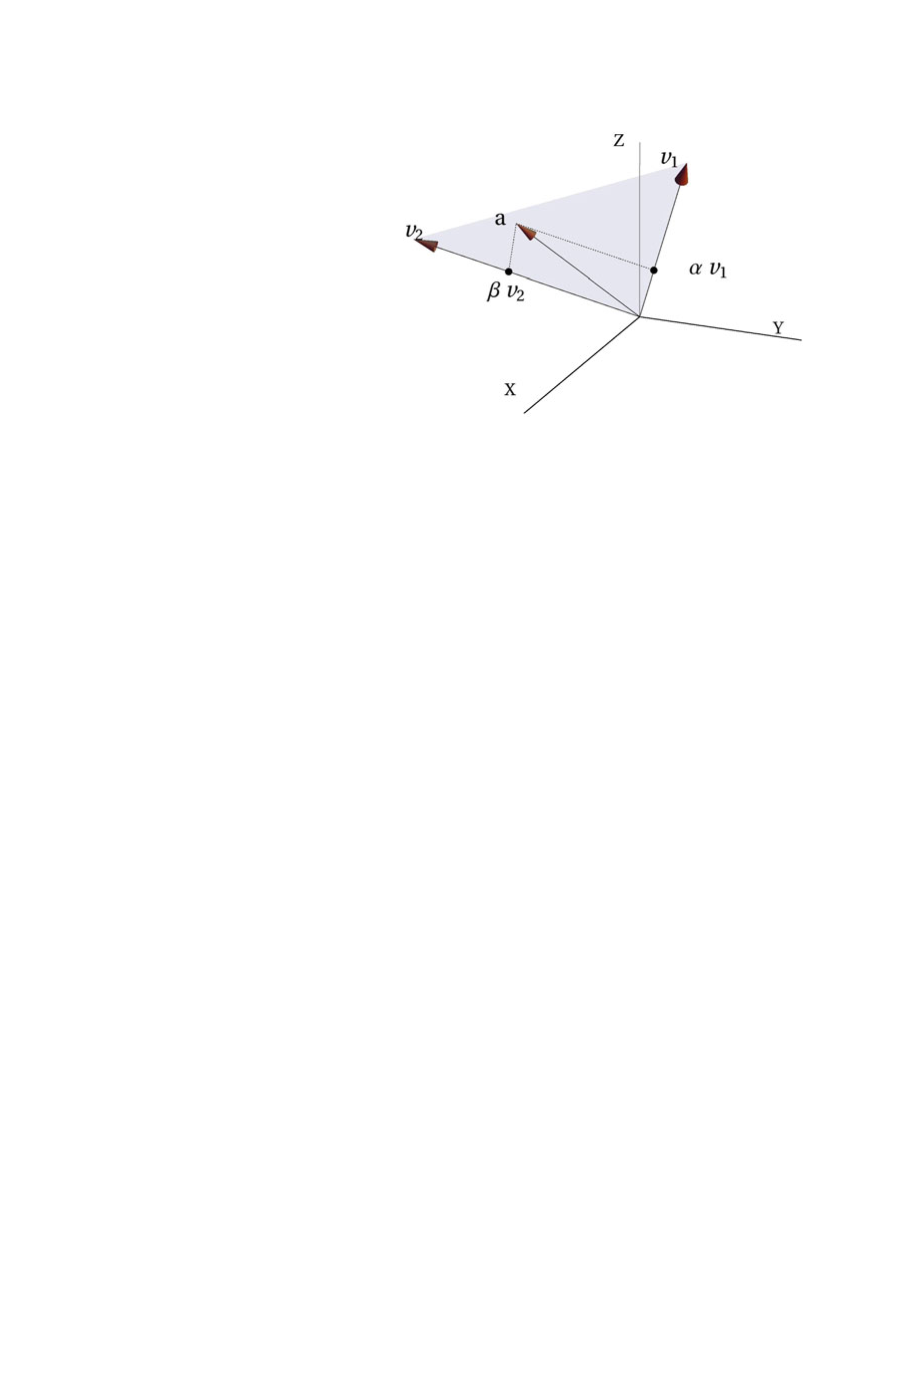
\includegraphics[width=0.5\linewidth]{fig_projection.pdf}
    \caption{الاسقاط التعامدي}
    \label{fig:enter-label}
\end{figure}

بالنظر إلى متجهين مستقلين خطيًا \( a \) و \( b \) في \( \mathbb{R}^n \), نريد إيجاد الإسقاط المتعامد لـ \( a \) على الخط الذي يتولده \( b \). لهذا الغرض, نرمز بـ \( M \) المستوي الذي يتولده \( a \) و \( b \) ونعتبر أساسًا متعامدًا { \( v_1 \), \( v_2 \) } لـ \( M \) يتكون من \( v_1 = \frac{b}{\|b\|} \) ومتجه وحدة \( v_2 \in M \) متعامد على \( v_1 \) (الشكل 1.1). بما أن { \( v_1 \), \( v_2 \) } هو أساس لـ \( M \), هناك أعداد حقيقية \( \alpha \) و \( \beta \) بحيث أن \( a = \alpha v_1 + \beta v_2 \).

الإسقاط لـ \( a \) على الخط الذي يتولده \( b \) هو بالتحديد \( \alpha v_1 \). لتحديد \( \alpha \), نأخذ ببساطة الجداء الداخلي مع \( b \) في الهوية أعلاه. بما أن \( \langle v_1, b \rangle = \|b\| \) و \( \langle v_2, b \rangle = 0 \), نحصل على:
أي أن,
\begin{eqnarray*}
\langle a, b \rangle = \alpha \|b\|.
\\
 \alpha = \frac{\langle a, b \rangle}{\|b\|}
\end{eqnarray*}
تمثل مركبة المتجه \( a \) الموازية للمتجه \( b \). سيكون هذا مفيدًا في الفصل 2 عندما نحسب مركبة القوة في الاتجاه المماسي لمسار معين. لاحظ أنه بهذه الطريقة, يمكننا فعليًا بناء أساس متعامد { \( v_1 \), \( v_2 \) } لـ \( M \) بأخذ:
\begin{eqnarray*}
 v_1 &:=& \frac{b}{\|b\|} \\
 v_2 &:=& \dfrac{a - \dfrac{\langle a, b \rangle}{\|b\|} \dfrac{b}{\|b\|}}{\|a - \dfrac{\langle a, b \rangle}{\|b\|} \frac{b}{\|b\|}\|}. 
\end{eqnarray*}
بالنظر إلى متجهين مستقلين خطيًا \( a \) و \( b \) في \( \mathbb{R}^n \), نريد إيجاد الإسقاط المتعامد لـ \( a \) على الخط الذي يتولده \( b \). لهذا الغرض, نرمز بـ \( M \) المستوي الذي يتولده \( a \) و \( b \) ونعتبر أساسًا متعامدًا { \( v_1 \), \( v_2 \) } لـ \( M \) يتكون من \( v_1 = \frac{b}{\|b\|} \) ومتجه وحدة \( v_2 \in M \) متعامد على \( v_1 \) (الشكل 1.1). بما أن { \( v_1 \), \( v_2 \) } هو أساس لـ \( M \), هناك أعداد حقيقية \( \alpha \) و \( \beta \) بحيث أن \( a = \alpha v_1 + \beta v_2 \).

الإسقاط لـ \( a \) على الخط الذي يتولده \( b \) هو بالتحديد \( \alpha v_1 \). لتحديد \( \alpha \), نأخذ ببساطة الجداء الداخلي مع \( b \) في الهوية أعلاه. بما أن \( \langle v_1, b \rangle = \|b\| \) و \( \langle v_2, b \rangle = 0 \), نحصل على:

أي أن,
\begin{eqnarray*}
\langle a, b \rangle = \alpha \|b\|.
\\
\alpha = \frac{\langle a, b \rangle}{\|b\|}
\end{eqnarray*}
تمثل مركبة المتجه \( a \) الموازية للمتجه \( b \). سيكون هذا مفيدًا في الفصل 2 عندما نحسب مركبة القوة في الاتجاه المماسي لمسار معين. لاحظ أنه بهذه الطريقة, يمكننا فعليًا بناء أساس متعامد { \( v_1 \), \( v_2 \) } لـ \( M \) بأخذ:

\begin{definition}
الضرب الاتجاهي لمتجهين
\[ a = (a_1, a_2, a_3) \text{ و } b = (b_1, b_2, b_3) \]
في \( \mathbb{R}^3 \) هو المتجه المعرف بالتعبير الرسمي

\[ a \times b := \begin{vmatrix} \mathbf{e}_1 & \mathbf{e}_2 & \mathbf{e}_3 \\ a_1 & a_2 & a_3 \\ b_1 & b_2 & b_3 \end{vmatrix}. \]

هنا, \(\{\mathbf{e}_1, \mathbf{e}_2, \mathbf{e}_3\}\) يمثل الأساس المعياري (الشكل 1.2) لـ \( \mathbb{R}^3 \), أي
\[ \mathbf{e}_1 = (1, 0, 0), \mathbf{e}_2 = (0, 1, 0), \mathbf{e}_3 = (0, 0, 1). \]
\end{definition}

ونفسر أن إحداثيات المتجه \( a \times b \) يتم الحصول عليها بعد توسيع المحدد على طول الصف الأول. أي أن,

\[ a \times b := \left( \begin{vmatrix} a_2 & a_3 \\ b_2 & b_3 \end{vmatrix}, -\begin{vmatrix} a_1 & a_3 \\ b_1 & b_3 \end{vmatrix}, \begin{vmatrix} a_1 & a_2 \\ b_1 & b_2 \end{vmatrix} \right). \]

إنها عملية حسابية روتينية ولكنها شاقة للتحقق من أن:

\[ \|a \times b\|^2 = \|a\|^2 \cdot \|b\|^2 - |\langle a, b \rangle|^2 = \|a\|^2 \cdot \|b\|^2 (1 - \cos^2(\theta)) = \|a\|^2 \cdot \|b\|^2 \sin^2(\theta), \]

حيث أن \( \theta \in [0, \pi] \) هي الزاوية بين المتجهين \( a \) و \( b \). بالتالي,

\[ \|a \times b\| = \|a\| \cdot \|b\| \cdot \sin(\theta). \]

\begin{figure}
    \centering
    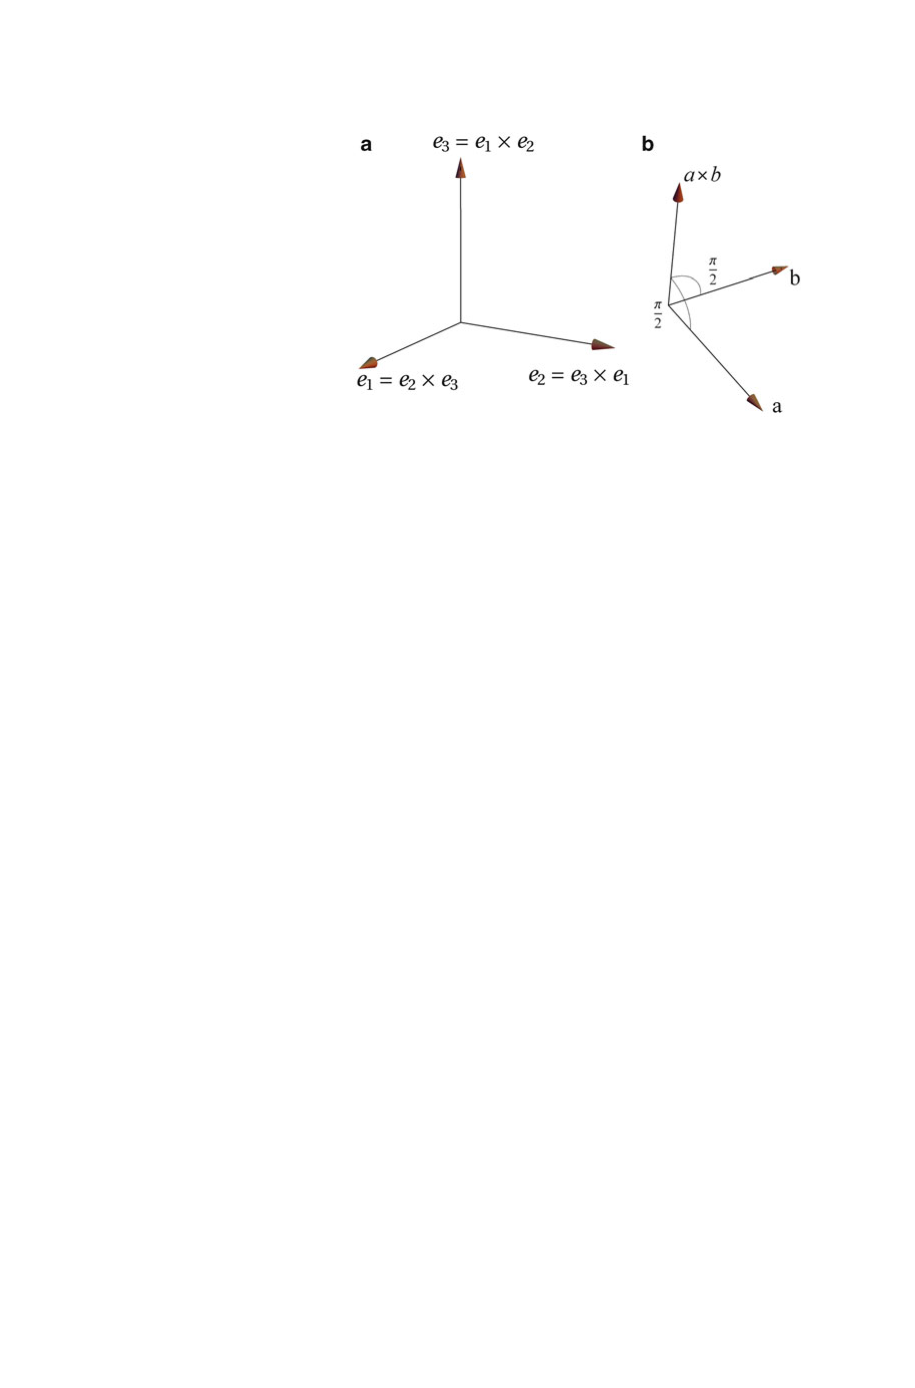
\includegraphics[width=0.5\linewidth]{cross_product.pdf}
    \caption{$(a)$ الاساس المعياري.  $(b)$ الضرب الاتجاهي}
    \label{fig:enter-label}
\end{figure}

إذا كان \( a \) و \( b \) مستقلين خطيًا, فإن هذا التعبير يعطي مساحة متوازي الأضلاع المتولد بواسطة \( a \) و \( b \) (انظر المثال 4.1.1).
\begin{definition}
حاصل الضرب الثلاثي القياسي لثلاثة متجهات \( a \), \( b \), و \( c \) في \( \mathbb{R}^3 \) هو العدد القياسي المعرف بـ
\[ \langle a, b \times c \rangle. \]
إذا كتبنا:
\[ a = (a_1, a_2, a_3), b = (b_1, b_2, b_3), c = (c_1, c_2, c_3), \]
فإنه يتبع من التعاريف أن:
\[ \langle a, b \times c \rangle = a_1 \begin{vmatrix} b_2 & b_3 \\ c_2 & c_3 \end{vmatrix} - a_2 \begin{vmatrix} b_1 & b_3 \\ c_1 & c_3 \end{vmatrix} + a_3 \begin{vmatrix} b_1 & b_2 \\ c_1 & c_2 \end{vmatrix} = \begin{vmatrix} a_1 & a_2 & a_3 \\ b_1 & b_2 & b_3 \\ c_1 & c_2 & c_3 \end{vmatrix}. \]
\end{definition}
من خواص المحددات, نحصل فورًا على الخواص التالية للضرب الاتجاهي لمتجهين.

\begin{theoreme}
يتمتع الضرب الاتجاهي بالخصائص التالية:
\begin{itemize}
    \item [(1)] \( b \times a = - (a \times b) \).
    \item [(2)] \( a \times b \) متعامد على المتجهين \( a \) و\( b \).
    \item [(3)] \( a \) و\( b \) مستقلان خطيًا إذا وفقط إذا كان \( a \times b \neq 0 \).
\end{itemize}
\end{theoreme}

الضرب الاتجاهي للمتجهات في \( \mathbb{R}^2 \) غير معرف. ومع ذلك, كما سنرى في القسم 7.2, من الممكن تعريف الضرب الاتجاهي لـ \( n - 1 \) متجهات في \( \mathbb{R}^n \) عندما يكون \( n \geq 3 \).
يتمتع حاصل الضرب الثلاثي القياسي أيضًا بتفسير هندسي مثير للاهتمام. لنفترض أن \( a \), \( b \), و\( c \in \mathbb{R}^3 \) هي ثلاثة متجهات مستقلة خطيًا. هذه المتجهات تولد متوازي مستطيلات, قاعدته يمكن أن تكون متوازي الأضلاع الذي يتولده \( a \) و\( b \) (انظر الشكل 1.3). المتجه \( a \times b \) متعامد على المستوى الذي يتولده \( a \) و\( b \), ونتيجة لذلك, ارتفاع هذا المتوازي المستطيلات (بالنسبة للمستوى المذكور) يتزامن مع مركبة \( c \) الموازية لاتجاه \( \pm (a \times b) \). أي أن الارتفاع يعطى بـ
\[ h = \left| \frac{\langle c, a \times b \rangle}{\|a \times b\|} \right|. \]
يمكن الآن حساب حجم متوازي المستطيلات عن طريق:
\[ الحجم = القاعدة \times الارتفاع = \|a \times b\| \cdot h = |\langle c, a \times b \rangle| = |\langle a, b \times c \rangle|. \]


\begin{figure}
    \centering
    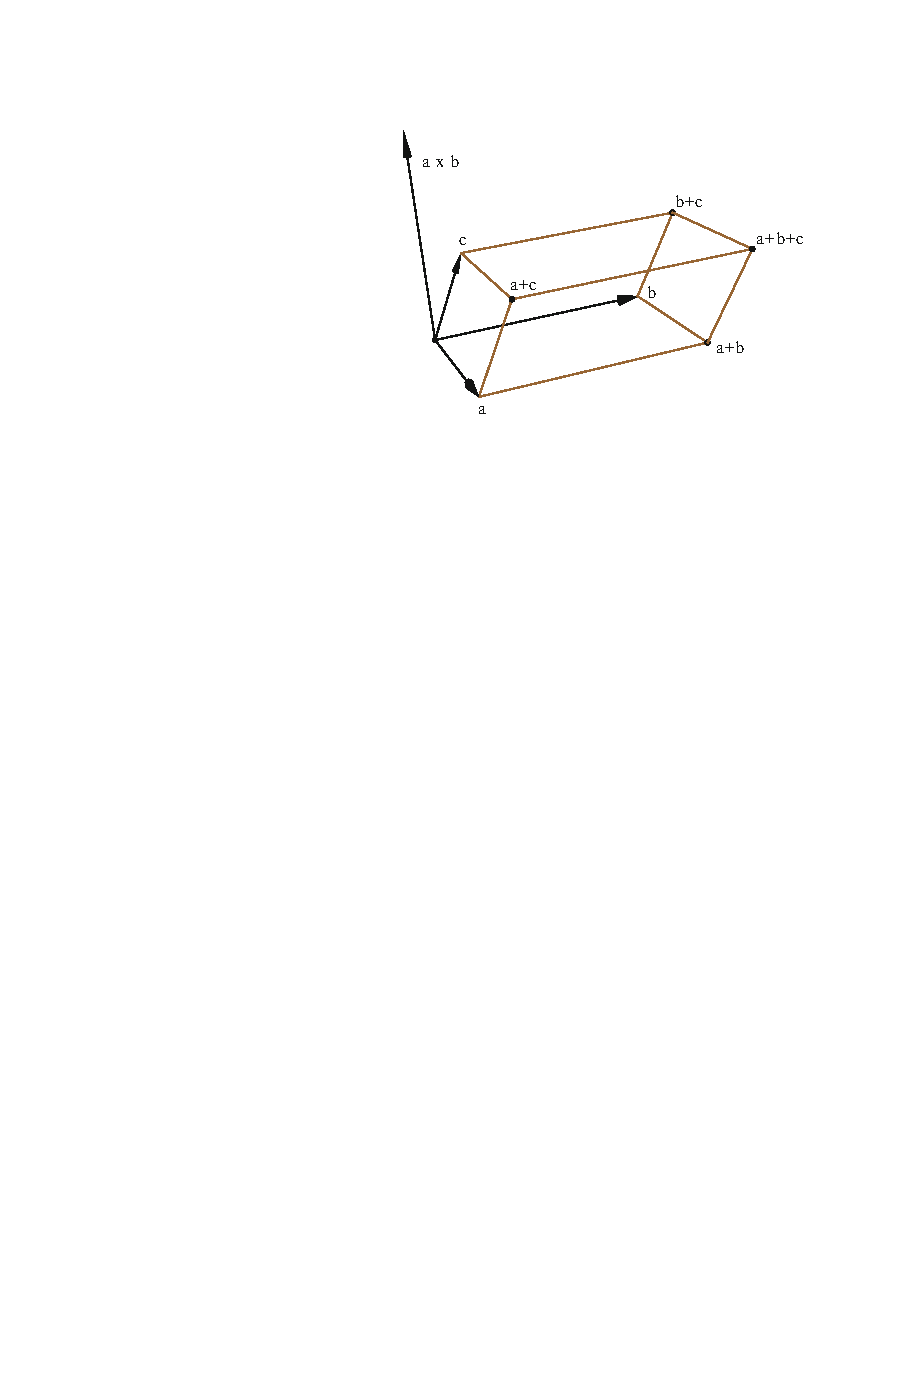
\includegraphics[width=0.5\linewidth]{Parallelepiped.pdf}
    \caption{متوازي مستطيلات يتولد بواسطة ثلاثة متجهات}
    \label{fig:enter-label}
\end{figure}

لذلك, حجم متوازي المستطيلات هو القيمة المطلقة لحاصل الضرب الثلاثي القياسي للمتجهات الثلاثة. سنعمم هذه النتيجة لاحقاً.
\newpage
\section{ الحقول المتجهة}

على مدار هذه الملخصات, نفترض أن الطالب لديه معرفة أساسية بالتفاضل والتكامل في عدة متغيرات, ولكن من أجل التناسق, سنستذكر التعريفات والنتائج ذات الصلة.

\begin{definition}
لنفترض أن \(a \in \mathbb{R}^n\), فإن الكرة المفتوحة ذات المركز \(a\) ونصف القطر \(r > 0\) هي المجموعة
\[ B(a, r) = \{x \in \mathbb{R}^n : \|x - a\| < r\}. \]
الكرة المغلقة ذات المركز \(a\) ونصف القطر \(r \geq 0\) هي المجموعة
\[ 
D(a, r) = \{x \in \mathbb{R}^n : \|x - a\| \leq r\}. 
\]
\end{definition}

\begin{definition}
\begin{itemize}
    \item [(i)] تُسمى مجموعة فرعية \(U\) من \(\mathbb{R}^n\) مفتوحة إذا لكل \(x \in U\) يوجد \(r > 0\) (يعتمد على \(x\)) بحيث \(B(x, r) \subset U\).
    \item [(ii)] تُسمى مجموعة \(C\) في \(\mathbb{R}^n\) مغلقة إذا كان متممها \(\mathbb{R}^n \setminus C\) مجموعة مفتوحة.
    \item [(iii)] لنفترض \(a \in \mathbb{R}^n\), تُسمى مجموعة \(G \subset \mathbb{R}^n\) حيًا لـ\(a\) إذا كان هناك \(r > 0\) بحيث تكون الكرة \(B(a, r)\) محتواة في \(G\). على وجه الخصوص, إذا كانت المجموعة \(G\) مفتوحة, فهي حي مفتوح لجميع نقاطها.
    \item[(iv)] إذا كانت \(A\) مجموعة فرعية من \(\mathbb{R}^n\), فإن داخل \(A\) هو المجموعة
    \[ 
    \operatorname{int}(A) := \{x \in A : A \text{ هو حي لـ } x\}.
    \]
    \item [(v)] إغلاق \(A\) هو المجموعة
    \[ 
    \bar{A} := \{x \in \mathbb{R}^n : B(x, r) \cap A \neq \emptyset \text{ لكل } r > 0\}. \]
\end{itemize}
\end{definition}

أي كرة مفتوحة \(B(a, r)\) هي مجموعة مفتوحة. في الواقع, إذا \(x \in B(a, r)\), فإن متباينات المثلث تعني أن \(B(x, r - \|x - a\|)\) هي كرة مفتوحة ذات المركز \(x\) محتواة في \(B(a, r)\). وبالمثل, فإن أي كرة مغلقة هي مجموعة مغلقة. بصفة عامة, مجموعة \(A\) مفتوحة إذا وفقط إذا كانت تتطابق مع داخلها, \(\operatorname{int}(A)\), وتكون مغلقة إذا وفقط إذا كانت تتطابق مع إغلاقها \(\bar{A}\).

نستذكر الآن مفاهيم الخرائط المستمرة والقابلة للتفاضل.

\begin{definition}
    
لنفترض أن \(M\) مجموعة فرعية من \(\mathbb{R}^n\). تخطيط \(f : M \subset \mathbb{R}^n \to \mathbb{R}^m\) تكون مستمرة عند نقطة \(a \in M\) إذا لكل \(\epsilon > 0\) يوجد \(\delta > 0\) بحيث لكل \(x \in M\) مع \(\|x - a\| < \delta\), لدينا
\[ \|f(x) - f(a)\| < \epsilon. \]
\end{definition}

نقول أن \(f\) مستمرة على \(M\) إذا كانت مستمرة عند كل نقطة من \(M\). عادةً عندما يكون مجال الصورة هو \(\mathbb{R}\) سنقول أن \(f\) دالة مستمرة.

\begin{definition}
لنفترض أن \(M\) مجموعة فرعية من \(\mathbb{R}^n\) ونعتبر \(a \in M\) التي تحتوي على خاصية أن \(M \cap (B(a, r) \setminus \{a\}) \neq \emptyset\) لكل \(r > 0\). نقول أن التخطيط \(f : M \subset \mathbb{R}^n \to \mathbb{R}^m\) لها حد \(b \in \mathbb{R}^m\) عند النقطة \(a\), ونكتب \(\lim_{x \to a} f(x) = b\), إذا لكل \(\epsilon > 0\) يوجد \(\delta > 0\) بحيث لكل \(x \in M\) مع \(\|x - a\| < \delta\), لدينا
\[ \|f(x) - b\| < \epsilon. \]
\end{definition}

\begin{definition}
    
لنفترض أن \(f : U \subset \mathbb{R}^n \to \mathbb{R}\) دالة معرفة على المجموعة المفتوحة \(U\). نقول أن \(f\) لديها مشتق جزئي في الإحداثي \(i\) عند \(a \in U\) إذا كان الحد
\[ \lim_{h \to 0} \frac{f(a_1, \ldots, a_{i-1}, a_i + h, a_{i+1}, \ldots, a_n) - f(a_1, \ldots, a_n)}{h} \]
موجودًا, وعندما يكون الحد موجودًا, سنرمز قيمته (وهو عدد حقيقي) بـ \(\frac{\partial f}{\partial x_i}(a)\).
\end{definition}

بصفة عامة, لـ \(f : U \subset \mathbb{R}^n \to \mathbb{R}^m\) و \(v \in \mathbb{R}^n\), نحدد المشتق الاتجاهي لـ \(f\) عند \(a \in U\) في الاتجاه \(v\) ليكون
\[ D_v f(a) = \lim_{t \to 0} \frac{f(a + tv) - f(a)}{t}, \]
عندما يكون هذا الحد موجودًا.

\begin{definition}
لنفترض أن \(f : U \subset \mathbb{R}^n \to \mathbb{R}^m\)تخطيط معرف  على المجموعة المفتوحة \(U\). نقول أن \(f\) قابلة للتفاضل عند \(a \in U\) إذا كانت هناك تخطيط خطي  \(T : \mathbb{R}^n \to \mathbb{R}^m\) بحيث
\[ \lim_{h \to 0} \frac{f(a + h) - f(a) - T(h)}{\|h\|} = 0. \]
في هذه الحالة, نرمز التخطيط الخطي الوحيد \(T\) بـ \(df(a)\). نقول أن \(f\) قابلة للتفاضل على \(U\) إذا كانت قابلة للتفاضل عند كل نقطة من \(U\).

تخطيط \(f : U \subset \mathbb{R}^n \to \mathbb{R}^m\), \(f = (f_1, \ldots, f_m)\), قابلة للتفاضل عند \(a \in U\) إذا وفقط إذا كانت كل دالة إحداثية \(f_j\) قابل للتفاضل عند \(a\). إذا رمزنا لمصفوفة \(df(a)\) (بالنسبة للأساس القانوني) بـ \(f'(a)\), يكون لدينا
\[ f'(a) = \begin{pmatrix}
\frac{\partial f_1}{\partial x_1}(a) & \frac{\partial f_1}{\partial x_2}(a) & \cdots & \frac{\partial f_1}{\partial x_n}(a) \\
\frac{\partial f_2}{\partial x_1}(a) & \frac{\partial f_2}{\partial x_2}(a) & \cdots & \frac{\partial f_2}{\partial x_n}(a) \\
\vdots & \vdots & \ddots & \vdots \\
\frac{\partial f_m}{\partial x_1}(a) & \frac{\partial f_m}{\partial x_2}(a) & \cdots & \frac{\partial f_m}{\partial x_n}(a)
\end{pmatrix}. \]
\end{definition}

 \(f'(a)\) تسمى
 مصفوفة الجاكوبيان او اليعقوبي لـ
\(f\) عند \(a\) وفي حالة \(m = n\), يُسمى محددها بـ يعقوبي لـ \(f\) عند \(a\) ويرمز له بـ \(J_f(a)\).

في حالة الدالة ذات القيمة العددية حيث \( f : U \subset \mathbb{R}^n \to \mathbb{R} \) قابلة للتفاضل عند \( a \), يُسمى \( f'(a) \) تدرج \( f \) عند \( a \). عادة ما يُرمز إليه بـ \( \nabla f(a) \) ويُعامل كمتجه صف في \( \mathbb{R}^n \), أي:
\[ \nabla f(a) = \left( \frac{\partial f}{\partial x_1} (a), \frac{\partial f}{\partial x_2} (a), \ldots, \frac{\partial f}{\partial x_n} (a) \right). \]

هي أنه إذا كانت الدالة \( f : U \subset \mathbb{R}^n \to \mathbb{R}^m \) قابلة للتفاضل عند \( a \in U \), فإن المشتقة الاتجاهية لـ \( f \) عند \( a \) في اتجاه \( v \) موجودة لكل \( v \in \mathbb{R}^n \) وتكون:
\[ D_v f(a) = df(a)(v). \]

الشرط للتفاضل المعطى في التعريف اعلاه ليس من السهل التحقق منه, ولكن النظرية التالية, التي يمكن العثور عليها في أي كتاب دراسي عن حساب التفاضل في عدة متغيرات, تقدم شرطًا كافيًا أكثر ملاءمة. نحتاج أولاً إلى تعريف آخر.

\begin{definition}
لنفترض أن \( f : U \subset \mathbb{R}^n \to \mathbb{R}^m \) دالة معرفة على المجموعة المفتوحة \( U \). نقول أن \( f \) قابلة للتفاضل باستمرار عند \( a \in U \) إذا كان هناك \( r > 0 \) بحيث تكون الكرة \( B(a, r) \) محتواة في \( U \) وجميع المشتقات الجزئية \( \frac{\partial f_i}{\partial x_j}(x) \) ( \( i = 1, \ldots, m \), \( j = 1, \ldots, n \) ) موجودة في الكرة ومستمرّة عند \( a \). ثم يُقال أن \( f \) من الفئة \( C^1 \) على \( U \) إذا كانت قابلة للتفاضل باستمرار عند جميع نقاط \( U \).
\end{definition}

\begin{theoreme}
إذا كانت \( f : U \subset \mathbb{R}^n \to \mathbb{R}^m \) دالة قابلة للتفاضل باستمرار عند نقطة \( a \) في مجموعة مفتوحة \( U \), فإن \( f \) قابلة للتفاضل عند \( a \). على وجه الخصوص, إذا كانت \( f \) من الفئة \( C^1 \) على المجموعة المفتوحة \( U \), فإن \( f \) قابلة للتفاضل على \( U \).
\end{theoreme}

إذا كانت \( f : U \subset \mathbb{R}^n \to \mathbb{R}^m \) دالة من الفئة \( C^1 \) على مجموعة مفتوحة \( U \), يمكننا النظر في الدوال المستمرة \( \frac{\partial f_i}{\partial x_j} : U \to \mathcal{R} \). سنقول أن \( f \) من الفئة \( C^2 \) على \( U \) إذا كانت كل \( \frac{\partial f_i}{\partial x_j} : U \to \mathcal{R} \) من الفئة \( C^1 \) على \( U \)
اذا كان كل
\[\frac{\partial f_i}{\partial x_j} : U \to \mathcal{R}\] 
هي فئة $C^1$ عل $U$, بمعني ان 
\[
\frac{\partial^2f_i}{\partial x_k \partial x_j}(x).
\]

يمكن بوضوح تكرار هذه العملية لتعريف دالة من الفئة \( C^p \) على \( U \). إذا كانت \( f \) من الفئة \( C^p \) لكل \( p \in \mathbb{N} \), فإننا نقول إنها من الفئة \( C^\infty \) على \( U \).

\begin{definition}
حقل المتجهات هو دالة مستمرة
\[ F : U \subset \mathbb{R}^n \to \mathbb{R}^n. \]
\end{definition}

\begin{figure}
    \centering
    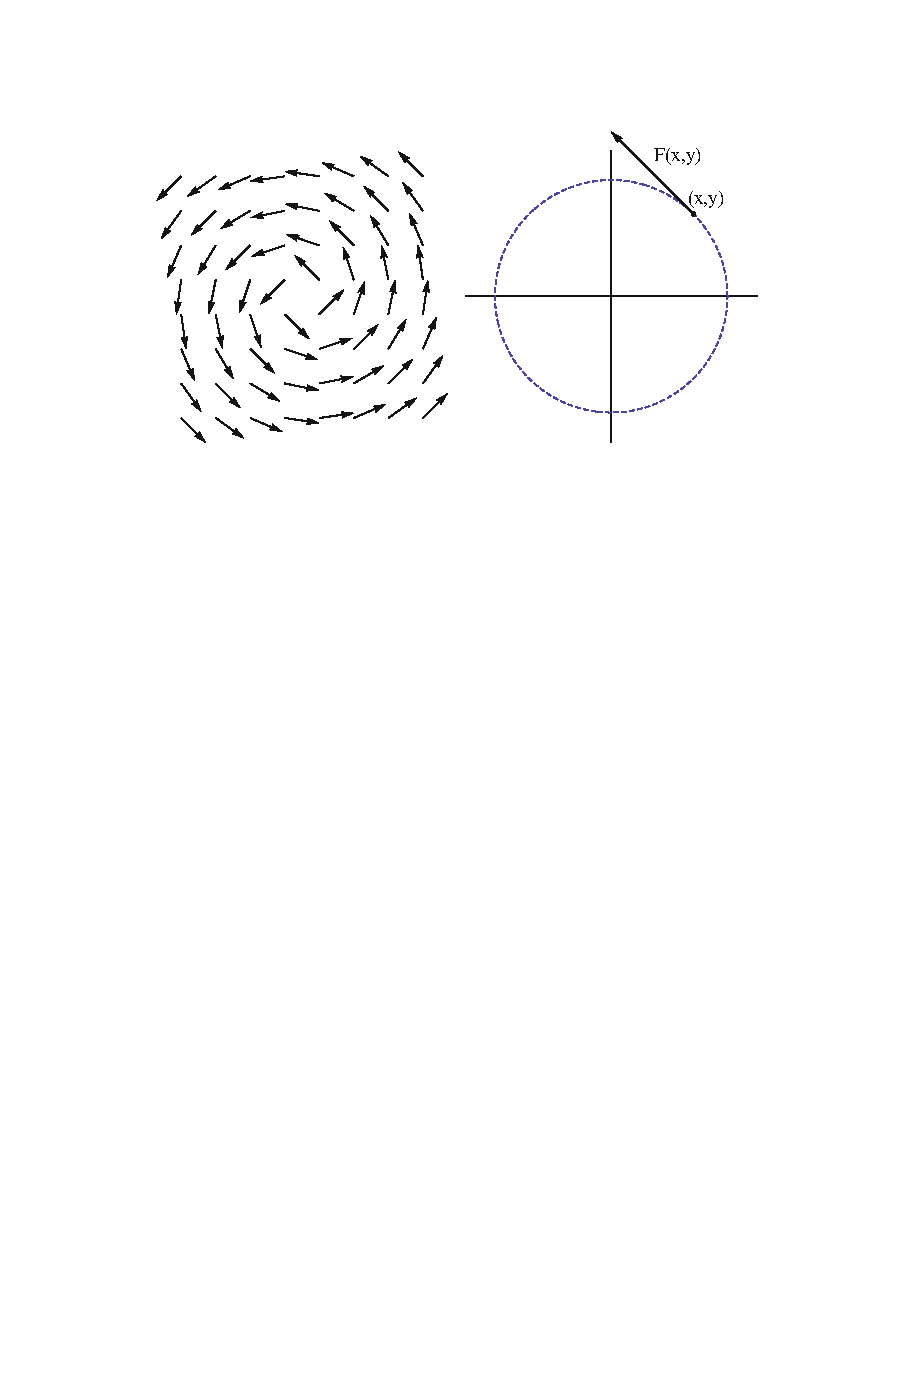
\includegraphics[width=0.8\linewidth]{vector field.pdf}
    \caption{مثال لحقل متحهات}
    \label{fig:enter-label}
\end{figure}

التفسير الطبيعي لهذا التعريف هو أن حقل المتجهات يخصص متجهًا لنقطة. حقول المتجهات مفيدة في تمثيل حقول القوة أو حقول السرعة. سيجد طالب الرياضيات في دراسته العديد من الحالات لهذا الموقف حيث يمكن تفسير نفس المفهوم المجرد بطرق مختلفة من خلال الجهاز البسيط لتغيير اسم ذلك المفهوم. هنا تصبح دالة من \( \mathbb{R}^n \) إلى نفسها مفهومًا فيزيائيًا, فقط من خلال تسميتها حقل متجهات, وبالتالي يتم تصورها بطريقة جديدة, كما توضح الأمثلة التالية.

\begin{exemple}
لننظر في حقل المتجهات (الشكل 1.4)
\[ F : \mathbb{R}^2 \setminus \{0\} \to \mathbb{R}^2 \]
المعرف بواسطة
\[ F(x, y) = \left( -\frac{y}{x^2 + y^2}, \frac{x}{x^2 + y^2} \right). \]

بوضوح, \( F(x, y) \) هو متجه وحدة, وإذا وضعنا هذا المتجه عند النقطة (x, y), نرى أنه متجه مماسي عند (x, y) للدائرة المتمركزة عند الأصل التي تمر بهذه النقطة.
\end{exemple}

\begin{exemple}[(حقول الجاذبية)]
لننظر في جسيم كتلته \( M \) موجود عند الأصل. قوة الجذب المؤثرة على جسيم كتلته \( m \) موجود عند \( (x, y, z) \in \mathbb{R}^3 \setminus \{0\} \) هي
\[ F(x, y, z) = - \frac{GMm}{(x^2 + y^2 + z^2)^{3/2}} (x, y, z), \]
حيث \( G \) هو ثابت الجاذبية و \( \mathbf{u} = \frac{(x, y, z)}{\sqrt{x^2 + y^2 + z^2}} \) هو متجه وحدة في الاتجاه من الأصل إلى (x, y, z). أي أن المتجه \( F(x, y, z) \) يشير دائمًا من (x, y, z) نحو الأصل, ومقداره يتناسب عكسيًا مع مربع المسافة إلى الأصل (الشكل 1.5).
\end{exemple}

\begin{figure}
    \centering
    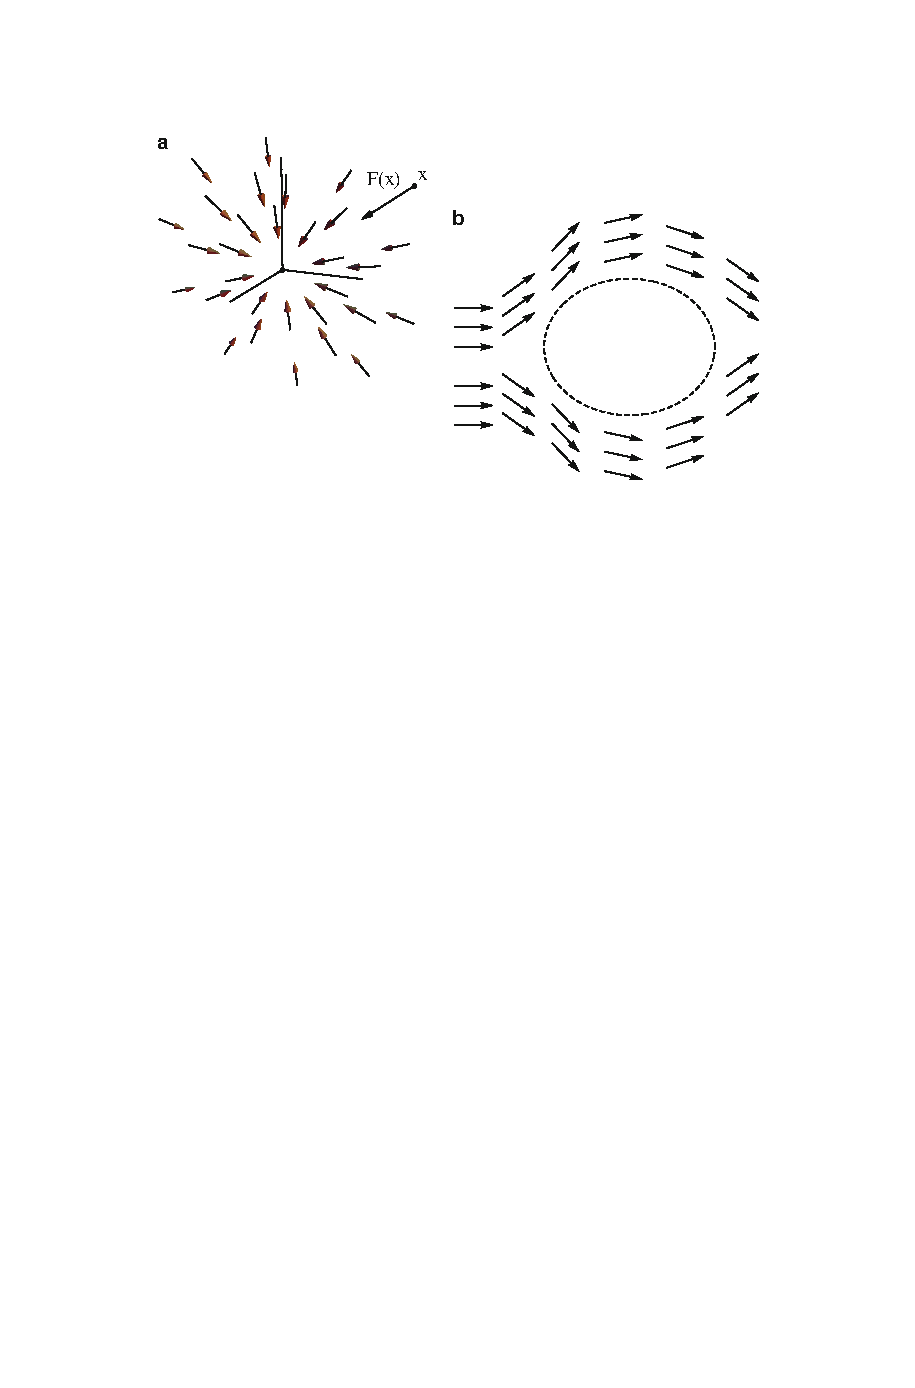
\includegraphics[width=0.8\linewidth]{Gravitational field.pdf}
    \caption{$a$  حقل متجهات        $b$ حركة جزي في مائع}
    \label{fig:enter-label}
\end{figure}

\begin{exemple}[(حقل السرعة لسائل)]

لكل نقطة \((x, y, z)\) من مجموعة مفتوحة \( U \subset \mathbb{R}^3 \) لنفترض أن \( F(x, y, z) \) تمثل سرعة سائل في الموضع \((x, y, z)\) عند زمن معين. إذن
\[ 
F : U \subset \mathbb{R}^3 \to \mathbb{R}^3 
\]
هو حقل متجهات.
\end{exemple}

\begin{exemple}

لنفترض أن
\[ g : U \subset \mathbb{R}^n \to \mathbb{R} \]
دالة من الفئة \( C^1 \) على المجموعة المفتوحة \( U \). إذن
\[ F := \nabla g : U \to \mathbb{R}^n, F(x) = \nabla g(x) := \left( \frac{\partial g}{\partial x_1}, \ldots, \frac{\partial g}{\partial x_n} \right) \]
هو حقل متجهات ويُسمى حقل التدرج لـ \( g \).
\end{exemple}

\begin{definition}
 
لنفترض أن \( \mathcal{F} : U \subset \mathbb{R}^n \to \mathbb{R}^n \) حقل متجهات بمكونات \( F = (f_1, f_2, \ldots, f_n) \). نتذكر أن \( F \) من الفئة \( C^p \) (أو قابل للتفاضل) على المجموعة المفتوحة \( U \) إذا كانت كل من مكوناته \( f_j \) من الفئة \( C^p \) (أو قابلة للتفاضل).
\end{definition}

بعد ذلك, نقدم عمليتين أساسيتين على حقول المتجهات؛ التباعد (وهو دالة عددية) والتدوير, أو الروتور (وهو حقل متجهات). يلعبان دورًا مركزيًا في صياغة نظريتين أساسيتين في التحليل المتجهي, وهما نظرية التباعد, أو نظرية غاوس, ونظرية ستوكس الكلاسيكية.  

\begin{definition}
لنفترض أن \( F : U \subset \mathbb{R}^n \to \mathbb{R}^n \) هو حقل متجهات من الفئة \( C^1 \) على المجموعة المفتوحة \( U \). التباعد \( \text{Div} \) لـ \( F \) هو الدالة العددية
\[ \text{Div} \, F = \sum_{j=1}^{n} \frac{\partial f_j}{\partial x_j}. \]
\end{definition}

\begin{definition}
لنفترض أن \( F : U \subset \mathbb{R}^3 \to \mathcal{R}^3, F = (f_1, f_2, f_3) \), هو حقل متجهات من الفئة \( C^1 \) على المجموعة المفتوحة \( U \). التدوير (أو الروتور) لـ \( F \) هو حقل المتجهات المعرف, رسميًا, بالمحدد
\begin{eqnarray*}
    \text{Curl} \, F = \begin{vmatrix} \mathbf{e}_1 & \mathbf{e}_2 & \mathbf{e}_3 \\ \frac{\partial}{\partial x} & \frac{\partial}{\partial y} & \frac{\partial}{\partial z} \\ 
    f_1 & f_2 & f_3 \end{vmatrix}. 
\end{eqnarray*}
\end{definition}

نفسر أن مكونات \( \text{Curl} \, F \) يتم الحصول عليها بعد توسيع المحدد على طول الصف الأول. وبالتالي, يكون \( \text{Curl} \, F \) هو حقل المتجهات

\begin{eqnarray*}
    \text{Curl} \, F &=& \left( \frac{\partial f_3}{\partial y} - \frac{\partial f_2}{\partial z}, \frac{\partial f_1}{\partial z} - \frac{\partial f_3}{\partial x}, \frac{\partial f_2}{\partial x} - \frac{\partial f_1}{\partial y} \right).
\end{eqnarray*}

عادةً ما نضع \( \nabla \) لتمثيل المؤثر التفاضلي

\[ \nabla = \left( \frac{\partial}{\partial x}, \frac{\partial}{\partial y}, \frac{\partial}{\partial z} \right). \]

هذا, مع ترميز الضرب الاتجاهي في التعريف 1.1.4, يقترح التمثيل الرمزي التالي لتدوير \( F \):

\[ \text{Curl} \, F = \nabla \times F. \]

نلاحظ أن التباعد معرّف لحقول المتجهات في \( \mathcal{R}^n \), بينما التدوير معرّف فقط لحقول المتجهات في \( \mathcal{R}^3 \).

\begin{figure}
    \centering
    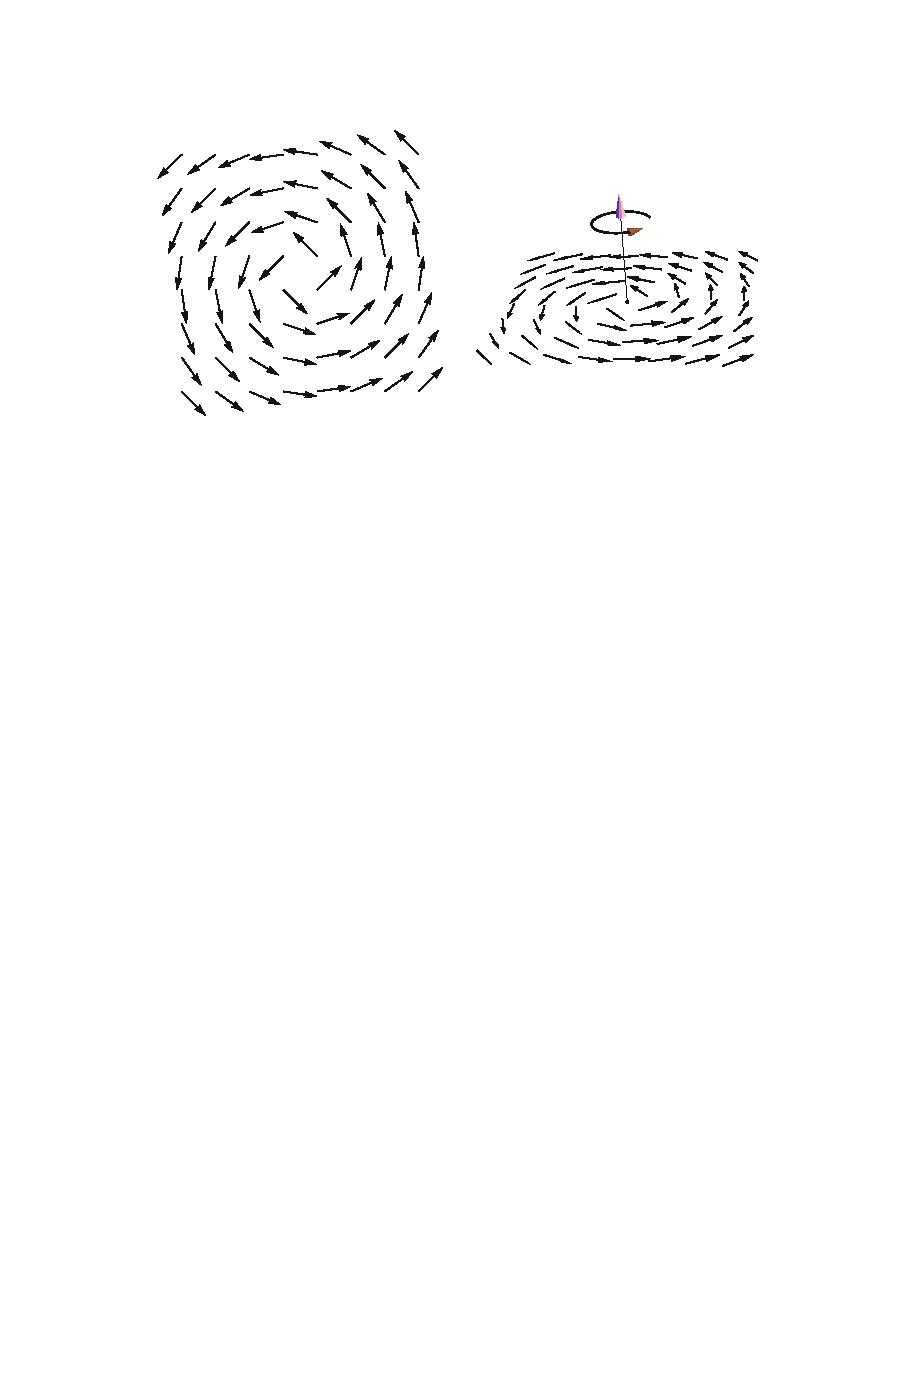
\includegraphics[width=0.8\linewidth]{Vector field Example.pdf}
    \caption{حقل متجهات}
    \label{fig:enter-label}
\end{figure}

\begin{exemple}
حقل المتجهات \( F(x, y, z) = (-y, x, 0) \) يمثل دورانًا حول \( N = (0, 0, 1) \). نلاحظ أن 
\( \text{Curl} \, F = (0, 0, 1) \) يعطي اتجاه محور الدوران (انظر الشكل 1.6). سنستنتج من نظرية ستوكس أن هذا ليس صدفة (انظر النتيجة 9.4.1).
\end{exemple}

بعد ذلك نسلط الضوء على علاقة مهمة بين التباعد والتدوير, ولكن لذلك, نحتاج إلى النظرية التالية المنسوبة إلى شوارتز حول تماثل المشتقات الثانية لدالة من الفئة \( C^2 \). يُطلق عليها أحيانًا أيضًا نظرية كليرو أو نظرية يونغ.

\begin{theoreme}
لنفترض أن \( f : U \subset \mathbb{R}^n \to \mathbb{R} \) دالة من الفئة \( C^2 \) على المجموعة المفتوحة \( U \). إذن, لكل \( x \in U \) ولكل \( i, j = 1, 2, \cdots, n \),
\[ 
\frac{\partial^2 f}{\partial x_i \partial x_j} (x) = \frac{\partial^2 f}{\partial x_j \partial x_i} (x). 
\]
\end{theoreme}

\begin{theoreme}

لنفترض أن \( F : U \subset \mathcal{R}^3 \to \mathcal{R}^3 \) هو حقل متجهات من الفئة \( C^2 \) على المجموعة المفتوحة \( U \). إذن,
\[
\text{Div} (\text{Curl} \, F) = 0.
\]
\end{theoreme}
\begin{demonstration}

نظرًا لأن \( F = (f_1, f_2, f_3) \), فإن نظرية شوارتز حول تماثل المشتقات الثانية تعطي:
\[ \text{Div} (\text{Curl} \, F) = \frac{\partial}{\partial x} \left( \frac{\partial f_3}{\partial y} - \frac{\partial f_2}{\partial z} \right) + \frac{\partial}{\partial y} \left( \frac{\partial f_1}{\partial z} - \frac{\partial f_3}{\partial x} \right) + \frac{\partial}{\partial z} \left( \frac{\partial f_2}{\partial x} - \frac{\partial f_1}{\partial y} \right). \]
باستخدام نظرية شوارتز نحصل على:
\[ = \frac{\partial^2 f_3}{\partial x \partial y} - \frac{\partial^2 f_2}{\partial x \partial z} + \frac{\partial^2 f_1}{\partial y \partial z} - \frac{\partial^2 f_3}{\partial y \partial x} + \frac{\partial^2 f_2}{\partial z \partial x} - \frac{\partial^2 f_1}{\partial z \partial y} = 0. \]
\end{demonstration}

    
\section{تمارين}

\begin{exercice}
 تحقق من أن
\[ \text{Div} (\text{Curl} F) = 0 \]
للحقل المتجه التالي:
\[ F(x, y, z) = (x^2z, x, 2yz) \]
\end{exercice}

\begin{exercice}
    احسب التباعد والدوران عند النقطة \((1, 1, 0)\) للحقل المتجه التالي:
\[ F(x, y, z) = (xyz, y, z). \]
\end{exercice}

\begin{exercice}
احسب التباعد للحقلين المتجهين التاليين:
\begin{enumerate}[start=3]
\item [1.] \( F(x, y) = (\sin(x), e^{x-y}) \).
\item [2.] \( F(x, y, z) = (\sin(y), \cos(z), z^3) \).
 \end{enumerate}
\end{exercice}

\begin{exercice}
    ليكن \( F : \mathbb{R}^3 \to \mathbb{R}^3 \) حقل متجه وليكن \( g : \mathbb{R}^3 \to \mathbb{R} \) دالة عددية, كلاهما من الفئة \( C^1 \) على \(\mathbb{R}^3\). تحقق من أن
\[ \text{Curl} (gF) = g(\text{Curl} F) + (\nabla g) \times F \].
\end{exercice}

\begin{exercice} 
إذا كانت \( F, G : \mathbb{R}^3 \to \mathbb{R}^3 \) حقول متجهة من الفئة \( C^1 \), أثبت أن
\[ \text{Div} (F \times G) = \langle \text{Curl} F, G \rangle - \langle F, \text{Curl} G \rangle \].
\end{exercice}
